% !TeX root = ../praktikum.tex
% !TeX encoding = UTF-8
% !Tex spellcheck = de_DE


Anhand der Messdaten aus der Gleichstrommessung, abgebildet in Graphik \ref{fig:full_range_dc} und \ref{fig:2T_range_dc}, wurde die Dichte der Ladungsträger im 2DEG, sowie deren Beweglichkeit bestimmt.

\subsubsection{Näherung über die Hall-Spannung}
\label{ch:naeherung_hall}

Zunächst wurde die Steigung der Hall-Spannung mittels linearer Regression aus dem klassischen Bereich der Messdaten zwischen \unit[-2]{T} und \unit[2]{T} anhand der Formel $ U_{Hall}=a\cdot B $  
bestimmt:
\begin{equation}
	a=\d{U_{Hall}}{B} = (1.876037 \pm 0,000305)\cdot10^{-3} ~  \unitfrac{m^2}{s}
\end{equation} %1.8760371604426e-03 +/- 3.0463451912632e-07

Hieraus ließ sich mit der Formel~\eqref{eq:ladungsdichte_steig} und dem bekannten Strom von $I=\unit[1]{\mu A}$ die Ladungsträgerdichte des 2DEG berechnen: 
\begin{equation}
	n_s= \frac{I}{e}\left({\d{U_{Hall}}{B}}\right)^{-1}=(3,33149 \pm 0,00054) ~ 10^{16}\cdot \unitfrac{1}{m^2}
\end{equation} %3,33149E+17	5,41062E+13
Mit den Bekannten Maßen der Probe wurde anschließend die Beweglichkeit der Ladungsträger bestimmt. Dies erfolgte anhand der Formel~\ref{eq:bewegl_masse} und mit der Probenlänge $L=600\mu m$ und -breite $W=100\mu m$.\\
\begin{equation}
\mu= (5,92433\pm 0,00096) ~ \unitfrac{m^2}{Vs} %5,92433E+06	9,62316E+02
\end{equation}


 
\subsubsection{Näherung über die Shubnikov-de Haas-Oszillation}
\label{ch:naeherung_sdho}

Eine Alternative Möglichkeit, die Ladungsträgerdichte zu berechnen, erfolgt über die Shubnikov-de Haas-Oszillation. Hierzu wurde die Längsspannung über der Probe 
%$U_{Längs}$
 gegen $\unitfrac{1}{B}$ aufgetragen und jedem Minimum der Oszillation ein Füllfaktor $\nu$ zugeordnet. Dies ist in Abbildung~\ref{fig:dc_sdho_ausw} zu sehen. Es wurde für den alle Minima die erste Messung verwendet (gesamter Messbereich), da die Auflösung ausreichend war. Ferner konnte so der leichte Versatz zwischen den Messungen keinen negativen Einfluss auf die Ergebnisse haben. Dafür wurde das Minimum/Plateau mit dem höchsten Füllfaktor, welches nur in der Teilbereichsmessung zu sehen war ignoriert.
 
Mit der linearen Regression $\mu = \nicefrac{b}{B}$ kann die Steigung zu $b=(13,1462 \pm 0,0190)\unit{T}$ bestimmt werden. Mit dieser ließ sich analog zur Näherung über die Hall-Spannung mit Gleichung~\eqref{eq:bewegl_masse} die Ladungsträgerdichte bestimmen:
\begin{equation}
n_s=  ( 3,17874 \pm 0,00046) \cdot 10^{15} ~ \unitfrac{1}{m^2}\\ %3,17874E+15	4,58225E+12
\end{equation}

So ergibt sich aus Gleichung~\eqref{eq:sdh_osz_naeherung} für die Beweglichkeit:
\begin{equation}
\mu= (6,20901\pm 0,00896) ~ \unitfrac{m^2}{Vs} %6,20901E+06	8,96337E+03
\end{equation}
 

\begin{figure}[h]
	\centering
	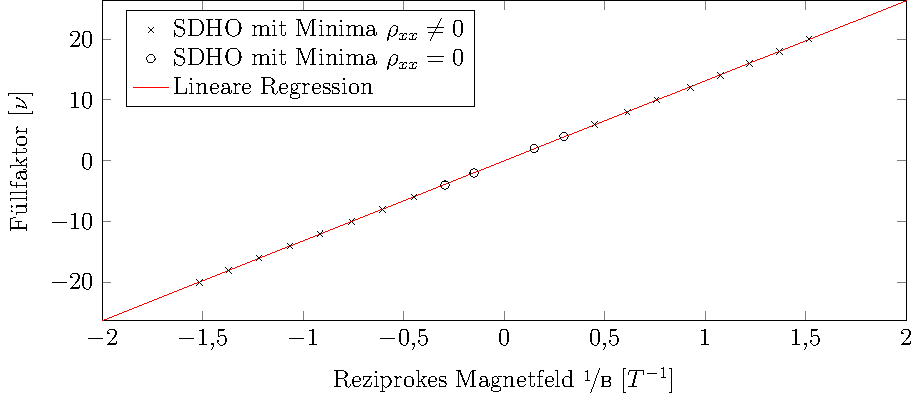
\includegraphics{graphs/dc/auswertung.pdf}
	\caption[Lineare Regression Gleichstrommessung]{
		Lineare Regression über den Füllfaktor der QHE-Plateaus der Gleichstrommessung aufgetragen gegen das Reziproke Magnetfeld.
	}
	\label{fig:dc_sdho_ausw}
\end{figure}

In den Graphen \ref{fig:full_range_dc} und \ref{fig:2T_range_dc} fiel eine leichte Asymmetrie der Messkurven auf. Da sich dies in allen folgenden Messungen ebenfalls bemerkbar machte, wurde hier auf einen Fehler an der Probe selbst geschlossen. So ist es zum Beispiel möglich, dass die Kontakte an der Probe zur Messung der Längs- und Hall-Spannungen eine leichte Asymmetrie aufweisen.

Wenn man über die Widerstandswerte des letzten Plateaus mit Füllfaktor $\nu = 2$ mittelt, kann man den Kitzling-Faktor errechnen:
$$ R_K = \unit[12,882 \pm 0,022]{k \Omega} \cdot 2 = \unit[25,764 \pm 0,044]{k \Omega}$$
Dieses Ergebnis liegt sehr dicht an dem Literaturwert von $R_K=\nicefrac{h}{e}=\unit[25,812]{k \Omega}$, wenngleich gerade eben nicht mehr im Konfidenzintervall. Dies könnte auf einen geringen Systematischen Fehler hinweisen. Um ein zuverlässigeres Ergebnis zu erhalten, müssten analog Rechnungen für weitere Plateaus durchgeführt werden. Dies wurde aus Zeitgründen in Rücksprache mit dem Betreuer nicht getan.